% !TeX program = pdflatex
\documentclass[11pt,a4paper]{article}
\usepackage[margin=19mm,headheight=14pt,headsep=9mm,footskip=10mm]{geometry}
\usepackage[T1]{fontenc}
\usepackage{lmodern}
\usepackage{amsmath,amssymb,array,booktabs,tabularx}
\usepackage{xcolor,tikz,fancyhdr}
\usepackage[hidelinks]{hyperref}
\definecolor{accent}{HTML}{245D91}
\definecolor{quiet}{HTML}{58616A}
\definecolor{wire}{HTML}{C8CDD2}
\setlength{\parindent}{0pt}
\setlength{\parskip}{5pt}
\renewcommand{\arraystretch}{1.15}
\pagestyle{fancy}
\fancyhf{}
\fancyhead[L]{\small\sffamily Word2Vec}
\fancyhead[R]{\small\sffamily Skip-gram with full Softmax}
\fancyfoot[R]{\small\thepage}
\renewcommand{\headrulewidth}{0.3pt}
\newcommand{\qa}[2]{%
  \par\addvspace{8pt}\noindent\textbf{#1}\par\nobreak
  \noindent #2\par}
\newcommand{\pagetitle}[1]{%
  {\Large\sffamily\bfseries #1}\par\medskip}
\newcolumntype{L}[1]{>{\raggedright\arraybackslash}p{#1}}
\hypersetup{
  pdftitle={Word2Vec: Structure and Questions},
  pdfsubject={A concise beginner guide to word vectors and Skip-gram training},
  pdfauthor={}
}

\begin{document}

{\LARGE\sffamily\bfseries Word2Vec: Structure and Questions}\par
{\color{quiet}A short guide based on our discussion.}\par
\medskip
\textbf{Scope.} The main example uses Skip-gram with full Softmax:
one center word predicts nearby context words.

\begin{center}
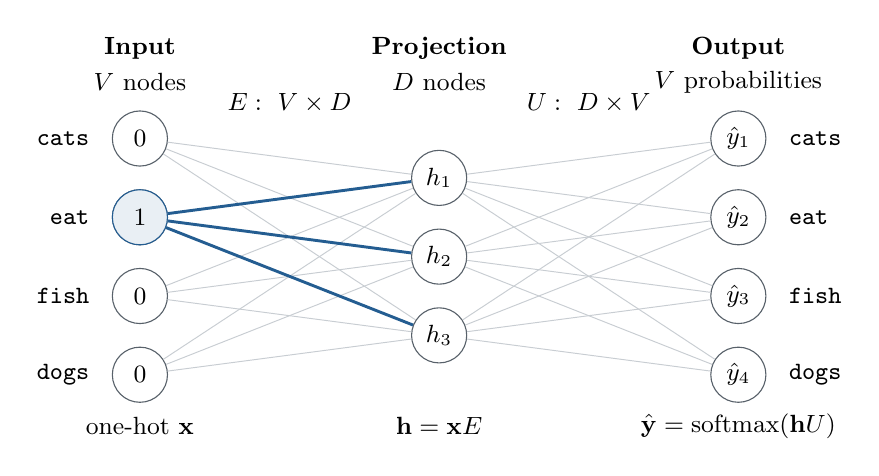
\begin{tikzpicture}[
  neuron/.style={circle,draw=quiet,fill=white,minimum size=7mm,inner sep=0pt},
  every node/.style={font=\small},
  link/.style={draw=wire,line width=0.35pt}
]
  \node[font=\small\bfseries] at (0,1.15) {Input};
  \node at (0,0.72) {$V$ nodes};
  \node[font=\small\bfseries] at (3.8,1.15) {Projection};
  \node at (3.8,0.72) {$D$ nodes};
  \node[font=\small\bfseries] at (7.6,1.15) {Output};
  \node at (7.6,0.72) {$V$ probabilities};

  \foreach \i/\yy/\val/\word in {
    1/0/0/cats,2/-1/1/eat,3/-2/0/fish,4/-3/0/dogs}{
    \node[neuron] (I\i) at (0,\yy) {$\val$};
    \node[anchor=east] at (-0.52,\yy) {\texttt{\word}};
    \node[neuron] (O\i) at (7.6,\yy) {$\hat y_{\i}$};
    \node[anchor=west] at (8.12,\yy) {\texttt{\word}};
  }
  \foreach \j/\yy in {1/-0.5,2/-1.5,3/-2.5}{
    \node[neuron] (H\j) at (3.8,\yy) {$h_{\j}$};
  }
  \foreach \i in {1,...,4}{
    \foreach \j in {1,...,3}{
      \draw[link] (I\i) -- (H\j);
      \draw[link] (H\j) -- (O\i);
    }
  }
  \foreach \j in {1,...,3}{
    \draw[accent,line width=1.05pt] (I2) -- (H\j);
  }
  \node[neuron,draw=accent,fill=accent!10] at (0,-1) {$1$};
  \node at (1.9,0.45) {$E:\ V\times D$};
  \node at (5.7,0.45) {$U:\ D\times V$};
  \node at (0,-3.65) {one-hot $\mathbf{x}$};
  \node at (3.8,-3.65) {$\mathbf{h}=\mathbf{x}E$};
  \node at (7.6,-3.65) {$\hat{\mathbf{y}}=\operatorname{softmax}(\mathbf{h}U)$};
\end{tikzpicture}

{\small Example: $V=4$, $D=3$, input = \texttt{eat}.
\textcolor{accent}{Blue connections} form the input word vector for \texttt{eat}.}
\end{center}

\begin{tabularx}{\linewidth}{@{}L{28mm}L{25mm}X@{}}
\toprule
Object & Size & Meaning \\
\midrule
Input $\mathbf{x}$ & $1\times V$ & One-hot vector identifying the center word. \\
Weights $E$ & $V\times D$ & Each row is one word's input embedding. \\
Hidden $\mathbf{h}$ & $1\times D$ & The selected embedding; one coordinate per node. \\
Weights $U$ & $D\times V$ & Each column is one word's output embedding. \\
Output $\hat{\mathbf{y}}$ & $1\times V$ & Probability of each word as a context word. \\
\bottomrule
\end{tabularx}

\medskip
\textbf{Why the weights are the word vectors.}
Rows of $E$ follow the vocabulary order. For illustration:
\[
E=
\begin{array}{c|rrr}
\texttt{cats}&0.1&0.3&-0.2\\
\texttt{eat}&0.2&-0.1&0.4\\
\texttt{fish}&-0.3&0.2&0.1\\
\texttt{dogs}&0.4&0.1&-0.1
\end{array}
\]
\[
\underbrace{[0,1,0,0]}_{\text{input: eat}}E
=0E_{\texttt{cats},:}+1E_{\texttt{eat},:}
 +0E_{\texttt{fish},:}+0E_{\texttt{dogs},:}
=[0.2,-0.1,0.4].
\]
One-hot multiplication selects one row. These three stored weights are the
input embedding of \texttt{eat}; the hidden activations equal that embedding.
This projection adds no bias or nonlinear activation.
Both $E$ and $U$ are trained; $E$ is commonly kept as the learned word vectors.

\clearpage
\pagetitle{Questions and short answers}

\qa{Q1. Is Word2Vec an embedding algorithm?}{
Yes. It learns static word embeddings.
Skip-gram predicts context words from a center word.
CBOW predicts a center word from surrounding words.}

\qa{Q2. Does the input layer have one node per vocabulary word?}{
Yes, in the one-hot view: its size is $V$.
In code, a word ID can directly select a row of $E$, without creating a long one-hot vector.}

\qa{Q3. Does one-hot represent the entire input sentence?}{
Here it identifies one center word.
A sentence supplies many center--context training pairs.}

\qa{Q4. What determines the number of hidden nodes?}{
We choose the embedding dimension $D$ before training.
It is a hyperparameter, independent of vocabulary size.
A larger $D$ uses more parameters and may need more data; it does not guarantee better results.}

\qa{Q5. How does a word correspond to a row of weights?}{
A fixed word-to-ID map assigns its row in $E$.
Training changes the numbers in that row.
For one input word, its $D$ outgoing weights form its input vector.}

\qa{Q6. What does the output layer predict?}{
It outputs $V$ probabilities: $\hat y_j=P(\text{context word }j\mid\text{center word})$.
They sum to 1.
The hidden layer holds the word vector; the output layer provides the prediction.}

\qa{Q7. Are there only two outputs, one for the previous and one for the next word?}{
There are $V$ output nodes.
A left/right window of size 1 can provide two training pairs.
Both pairs use the same output layer and weights.}

\qa{Q8. Is the output also one-hot?}{
The prediction is a probability vector, such as $[0.45,0.10,0.45]$.
A single training pair has a one-hot target, such as $[1,0,0]$.
The target can also be stored as a word ID.}

\qa{Q9. Does Skip-gram predict the next word?}{
Its targets include words on both sides within the chosen window.
Basic Skip-gram uses the same distribution for these positions.
Predicting only the next word is a different training objective.}

\clearpage
\pagetitle{Examples, boundaries, and training}

\qa{Q10. For \texttt{cats eat fish}, what are the inputs, targets, and boundaries?}{
Use vocabulary $[\texttt{cats},\texttt{eat},\texttt{fish}]$
and a window of one word on each side.
The complete set of training pairs is:}

\begin{center}
\begin{tabular}{@{}llll@{}}
\toprule
Center & Input $\mathbf{x}$ & Context target & Target $\mathbf{y}$ \\
\midrule
\texttt{cats} & $[1,0,0]$ & \texttt{eat}  & $[0,1,0]$ \\
\texttt{eat}  & $[0,1,0]$ & \texttt{cats} & $[1,0,0]$ \\
\texttt{eat}  & $[0,1,0]$ & \texttt{fish} & $[0,0,1]$ \\
\texttt{fish} & $[0,0,1]$ & \texttt{eat}  & $[0,1,0]$ \\
\bottomrule
\end{tabular}
\end{center}

At sentence boundaries, use only neighbors that exist.
Here, \texttt{cats} and \texttt{fish} each provide one pair;
\texttt{eat} provides two. No padding is needed.
For \texttt{eat}, the ideal output on this toy data approaches
$[0.5,0,0.5]$.
An actual finite Softmax output has strictly positive entries.

\qa{Q11. What if the data also contains \texttt{dogs eat meat}?}{
Expand the vocabulary to
$[\texttt{cats},\texttt{eat},\texttt{fish},\texttt{dogs},\texttt{meat}]$.
For center \texttt{eat}, the four targets are
\texttt{cats}, \texttt{fish}, \texttt{dogs}, and \texttt{meat}.}

If each sentence occurs once, the ideal distribution for \texttt{eat} is
\[
[1/4,\ 0,\ 1/4,\ 1/4,\ 1/4].
\]
If \texttt{cats eat fish} occurs three times and \texttt{dogs eat meat} once, it is
\[
[3/8,\ 0,\ 3/8,\ 1/8,\ 1/8].
\]
These are idealized frequencies for equally weighted pairs with the fixed window.
The input \texttt{eat} gives the same distribution in both sentences:
this model receives only the center word.

\qa{Q12. Are the training targets obtained from statistics over large text data?}{
We choose the task and window; the text supplies each pair's correct answer.
Repeated training learns the context statistics.
We do not need to precompute a complete probability table.}

For $N$ pairs $(w_k,c_k)$, minimize the average cross-entropy loss:
\[
\mathcal{L}=-\frac{1}{N}\sum_{k=1}^{N}\log P(c_k\mid w_k).
\]
Backpropagation computes gradients. An optimizer updates $E$ and $U$.
The vectors typically start from small random values and learn through these updates.

\medskip
{\small\color{quiet}
\textbf{Sources.}
\href{https://arxiv.org/abs/1301.3781}{Mikolov et al., Word2Vec architectures (2013)};
\href{https://arxiv.org/abs/1310.4546}{Mikolov et al., Skip-gram formulation (2013)};
\href{https://docs.pytorch.org/tutorials/beginner/nlp/word_embeddings_tutorial.html}{PyTorch, Word Embeddings tutorial}.
}
\end{document}
